\documentclass[twoside]{book}

% Packages required by doxygen
\usepackage{fixltx2e}
\usepackage{calc}
\usepackage{doxygen}
\usepackage[export]{adjustbox} % also loads graphicx
\usepackage{graphicx}
\usepackage[utf8]{inputenc}
\usepackage{makeidx}
\usepackage{multicol}
\usepackage{multirow}
\PassOptionsToPackage{warn}{textcomp}
\usepackage{textcomp}
\usepackage[nointegrals]{wasysym}
\usepackage[table]{xcolor}

% Font selection
\usepackage[T1]{fontenc}
\usepackage[scaled=.90]{helvet}
\usepackage{courier}
\usepackage{amssymb}
\usepackage{sectsty}
\renewcommand{\familydefault}{\sfdefault}
\allsectionsfont{%
  \fontseries{bc}\selectfont%
  \color{darkgray}%
}
\renewcommand{\DoxyLabelFont}{%
  \fontseries{bc}\selectfont%
  \color{darkgray}%
}
\newcommand{\+}{\discretionary{\mbox{\scriptsize$\hookleftarrow$}}{}{}}

% Page & text layout
\usepackage{geometry}
\geometry{%
  a4paper,%
  top=2.5cm,%
  bottom=2.5cm,%
  left=2.5cm,%
  right=2.5cm%
}
\tolerance=750
\hfuzz=15pt
\hbadness=750
\setlength{\emergencystretch}{15pt}
\setlength{\parindent}{0cm}
\setlength{\parskip}{3ex plus 2ex minus 2ex}
\makeatletter
\renewcommand{\paragraph}{%
  \@startsection{paragraph}{4}{0ex}{-1.0ex}{1.0ex}{%
    \normalfont\normalsize\bfseries\SS@parafont%
  }%
}
\renewcommand{\subparagraph}{%
  \@startsection{subparagraph}{5}{0ex}{-1.0ex}{1.0ex}{%
    \normalfont\normalsize\bfseries\SS@subparafont%
  }%
}
\makeatother

% Headers & footers
\usepackage{fancyhdr}
\pagestyle{fancyplain}
\fancyhead[LE]{\fancyplain{}{\bfseries\thepage}}
\fancyhead[CE]{\fancyplain{}{}}
\fancyhead[RE]{\fancyplain{}{\bfseries\leftmark}}
\fancyhead[LO]{\fancyplain{}{\bfseries\rightmark}}
\fancyhead[CO]{\fancyplain{}{}}
\fancyhead[RO]{\fancyplain{}{\bfseries\thepage}}
\fancyfoot[LE]{\fancyplain{}{}}
\fancyfoot[CE]{\fancyplain{}{}}
\fancyfoot[RE]{\fancyplain{}{\bfseries\scriptsize Generated by Doxygen }}
\fancyfoot[LO]{\fancyplain{}{\bfseries\scriptsize Generated by Doxygen }}
\fancyfoot[CO]{\fancyplain{}{}}
\fancyfoot[RO]{\fancyplain{}{}}
\renewcommand{\footrulewidth}{0.4pt}
\renewcommand{\chaptermark}[1]{%
  \markboth{#1}{}%
}
\renewcommand{\sectionmark}[1]{%
  \markright{\thesection\ #1}%
}

% Indices & bibliography
\usepackage{natbib}
\usepackage[titles]{tocloft}
\setcounter{tocdepth}{3}
\setcounter{secnumdepth}{5}
\makeindex

% Hyperlinks (required, but should be loaded last)
\usepackage{ifpdf}
\ifpdf
  \usepackage[pdftex,pagebackref=true]{hyperref}
\else
  \usepackage[ps2pdf,pagebackref=true]{hyperref}
\fi
\hypersetup{%
  colorlinks=true,%
  linkcolor=blue,%
  citecolor=blue,%
  unicode%
}

% Custom commands
\newcommand{\clearemptydoublepage}{%
  \newpage{\pagestyle{empty}\cleardoublepage}%
}

\usepackage{caption}
\captionsetup{labelsep=space,justification=centering,font={bf},singlelinecheck=off,skip=4pt,position=top}

%===== C O N T E N T S =====

\begin{document}

% Titlepage & ToC
\hypersetup{pageanchor=false,
             bookmarksnumbered=true,
             pdfencoding=unicode
            }
\pagenumbering{alph}
\begin{titlepage}
\vspace*{7cm}
\begin{center}%
{\Large Image\+Recognition \\[1ex]\large 0.\+1 }\\
\vspace*{1cm}
{\large Generated by Doxygen 1.8.13}\\
\end{center}
\end{titlepage}
\clearemptydoublepage
\pagenumbering{roman}
\tableofcontents
\clearemptydoublepage
\pagenumbering{arabic}
\hypersetup{pageanchor=true}

%--- Begin generated contents ---
\chapter{Namespace Index}
\section{Namespace List}
Here is a list of all namespaces with brief descriptions\+:\begin{DoxyCompactList}
\item\contentsline{section}{\hyperlink{namespace_controller}{Controller} }{\pageref{namespace_controller}}{}
\item\contentsline{section}{\hyperlink{namespace_controller_1_1_controlador}{Controller.\+Controlador} }{\pageref{namespace_controller_1_1_controlador}}{}
\item\contentsline{section}{\hyperlink{namespace_controller_1_1_controlador_prueba_unitaria}{Controller.\+Controlador\+Prueba\+Unitaria} }{\pageref{namespace_controller_1_1_controlador_prueba_unitaria}}{}
\item\contentsline{section}{\hyperlink{namespace_controller_1_1_gestor_general}{Controller.\+Gestor\+General} }{\pageref{namespace_controller_1_1_gestor_general}}{}
\item\contentsline{section}{\hyperlink{namespace_controller_1_1_gestor_sujeto}{Controller.\+Gestor\+Sujeto} }{\pageref{namespace_controller_1_1_gestor_sujeto}}{}
\item\contentsline{section}{\hyperlink{namespace_controller_1_1main}{Controller.\+main} }{\pageref{namespace_controller_1_1main}}{}
\item\contentsline{section}{\hyperlink{namespacedocstring}{docstring} \\*Created on Aug 16, 2017 }{\pageref{namespacedocstring}}{}
\end{DoxyCompactList}

\chapter{Hierarchical Index}
\section{Class Hierarchy}
This inheritance list is sorted roughly, but not completely, alphabetically\+:\begin{DoxyCompactList}
\item object\begin{DoxyCompactList}
\item \contentsline{section}{Controller.\+Controlador.\+Controlador}{\pageref{class_controller_1_1_controlador_1_1_controlador}}{}
\item \contentsline{section}{Controller.\+Gestor\+General.\+Gestor\+General}{\pageref{class_controller_1_1_gestor_general_1_1_gestor_general}}{}
\begin{DoxyCompactList}
\item \contentsline{section}{Controller.\+Gestor\+Sujeto.\+Gestor\+Sujeto}{\pageref{class_controller_1_1_gestor_sujeto_1_1_gestor_sujeto}}{}
\end{DoxyCompactList}
\item \contentsline{section}{Model.\+Sujeto.\+Sujeto}{\pageref{class_model_1_1_sujeto_1_1_sujeto}}{}
\end{DoxyCompactList}
\item Test\+Case\begin{DoxyCompactList}
\item \contentsline{section}{Controller.\+Controlador\+Prueba\+Unitaria.\+Controlador\+Test}{\pageref{class_controller_1_1_controlador_prueba_unitaria_1_1_controlador_test}}{}
\end{DoxyCompactList}
\end{DoxyCompactList}

\chapter{Class Index}
\section{Class List}
Here are the classes, structs, unions and interfaces with brief descriptions\+:\begin{DoxyCompactList}
\item\contentsline{section}{\hyperlink{class_controller_1_1_controlador_1_1_controlador}{Controller.\+Controlador.\+Controlador} \\*Clase controlador }{\pageref{class_controller_1_1_controlador_1_1_controlador}}{}
\item\contentsline{section}{\hyperlink{class_controller_1_1_gestor_general_1_1_gestor_general}{Controller.\+Gestor\+General.\+Gestor\+General} }{\pageref{class_controller_1_1_gestor_general_1_1_gestor_general}}{}
\item\contentsline{section}{\hyperlink{class_controller_1_1_gestor_sujeto_1_1_gestor_sujeto}{Controller.\+Gestor\+Sujeto.\+Gestor\+Sujeto} }{\pageref{class_controller_1_1_gestor_sujeto_1_1_gestor_sujeto}}{}
\end{DoxyCompactList}

\chapter{Namespace Documentation}
\hypertarget{namespace_controller_1_1_controlador_prueba_unitaria}{}\section{Controller.\+Controlador\+Prueba\+Unitaria Namespace Reference}
\label{namespace_controller_1_1_controlador_prueba_unitaria}\index{Controller.\+Controlador\+Prueba\+Unitaria@{Controller.\+Controlador\+Prueba\+Unitaria}}
\subsection*{Classes}
\begin{DoxyCompactItemize}
\item 
class \hyperlink{class_controller_1_1_controlador_prueba_unitaria_1_1_controlador_test}{Controlador\+Test}
\end{DoxyCompactItemize}


\subsection{Detailed Description}
\begin{DoxyVerb}Created on Aug 19, 2017

@author: HP
\end{DoxyVerb}
 
\hypertarget{namespace_controller_1_1_gestor_general}{}\section{Controller.\+Gestor\+General Namespace Reference}
\label{namespace_controller_1_1_gestor_general}\index{Controller.\+Gestor\+General@{Controller.\+Gestor\+General}}
\subsection*{Classes}
\begin{DoxyCompactItemize}
\item 
class \hyperlink{class_controller_1_1_gestor_general_1_1_gestor_general}{Gestor\+General}
\end{DoxyCompactItemize}


\subsection{Detailed Description}
\begin{DoxyVerb}Created on Aug 16, 2017

@author: HP
\end{DoxyVerb}
 
\hypertarget{namespace_controller_1_1_gestor_sujeto}{}\section{Controller.\+Gestor\+Sujeto Namespace Reference}
\label{namespace_controller_1_1_gestor_sujeto}\index{Controller.\+Gestor\+Sujeto@{Controller.\+Gestor\+Sujeto}}
\subsection*{Classes}
\begin{DoxyCompactItemize}
\item 
class \hyperlink{class_controller_1_1_gestor_sujeto_1_1_gestor_sujeto}{Gestor\+Sujeto}
\begin{DoxyCompactList}\small\item\em Clase \hyperlink{class_controller_1_1_gestor_sujeto_1_1_gestor_sujeto}{Gestor\+Sujeto}. \end{DoxyCompactList}\end{DoxyCompactItemize}

\hypertarget{namespacedocstring}{}\section{docstring Namespace Reference}
\label{namespacedocstring}\index{docstring@{docstring}}


Created on Aug 16, 2017.  




\subsection{Detailed Description}
Created on Aug 16, 2017. 

\begin{DoxyAuthor}{Author}
Michael Choque 
\end{DoxyAuthor}

\chapter{Class Documentation}
\hypertarget{class_controller_1_1_controlador_1_1_controlador}{}\section{Controller.\+Controlador.\+Controlador Class Reference}
\label{class_controller_1_1_controlador_1_1_controlador}\index{Controller.\+Controlador.\+Controlador@{Controller.\+Controlador.\+Controlador}}


Clase controlador.  


Inheritance diagram for Controller.\+Controlador.\+Controlador\+:\begin{figure}[H]
\begin{center}
\leavevmode
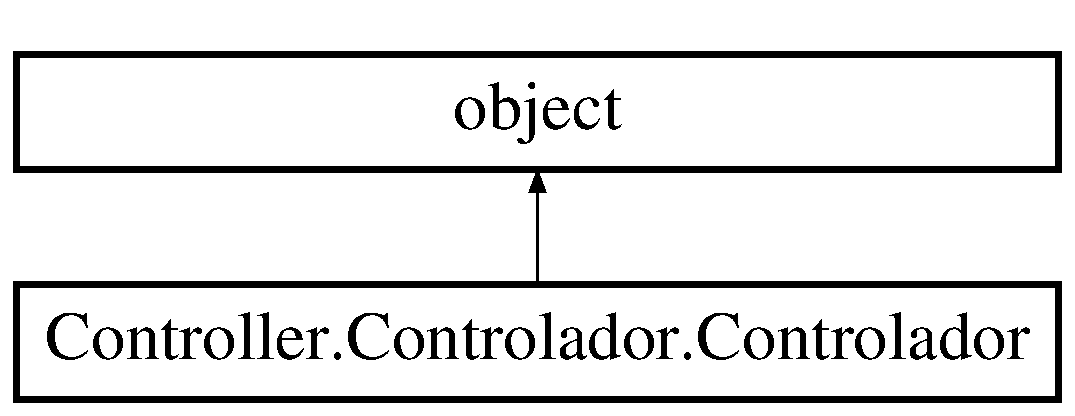
\includegraphics[height=2.000000cm]{class_controller_1_1_controlador_1_1_controlador}
\end{center}
\end{figure}
\subsection*{Public Member Functions}
\begin{DoxyCompactItemize}
\item 
def \hyperlink{class_controller_1_1_controlador_1_1_controlador_ad30f895c86fb2085fbd3b2c0a1c9f38c}{\+\_\+\+\_\+init\+\_\+\+\_\+} (self)
\begin{DoxyCompactList}\small\item\em Constructor de la clase. \end{DoxyCompactList}\item 
def \hyperlink{class_controller_1_1_controlador_1_1_controlador_a4bbeb1232cf73c6c9113e7ffda714b63}{Vectorizar\+Imagen} (self, img)
\item 
def \hyperlink{class_controller_1_1_controlador_1_1_controlador_a88254f919a6b1d7ed25e2f54b528a15c}{Definir\+Matriz\+De\+Imagenes} (self, list\+Imgs)
\item 
def \hyperlink{class_controller_1_1_controlador_1_1_controlador_a4c342a4b7f56c2f8a566cdf62030816c}{Definir\+Matriz\+De\+Covarianza} (self, matriz\+Img\+Vec)
\begin{DoxyCompactList}\small\item\em Metodo Definir\+Matriz\+De\+Covarianza. \end{DoxyCompactList}\end{DoxyCompactItemize}
\subsection*{Public Attributes}
\begin{DoxyCompactItemize}
\item 
\hyperlink{class_controller_1_1_controlador_1_1_controlador_ac7f14b4e1c0f2bf39ef0ddf2ae687898}{lista\+De\+Sujetos}
\end{DoxyCompactItemize}


\subsection{Detailed Description}
Clase controlador. 

Esta clase es la que permite la comunicacion entre los datos de la aplicacion y la interfaz de usuario 

\subsection{Constructor \& Destructor Documentation}
\mbox{\Hypertarget{class_controller_1_1_controlador_1_1_controlador_ad30f895c86fb2085fbd3b2c0a1c9f38c}\label{class_controller_1_1_controlador_1_1_controlador_ad30f895c86fb2085fbd3b2c0a1c9f38c}} 
\index{Controller\+::\+Controlador\+::\+Controlador@{Controller\+::\+Controlador\+::\+Controlador}!\+\_\+\+\_\+init\+\_\+\+\_\+@{\+\_\+\+\_\+init\+\_\+\+\_\+}}
\index{\+\_\+\+\_\+init\+\_\+\+\_\+@{\+\_\+\+\_\+init\+\_\+\+\_\+}!Controller\+::\+Controlador\+::\+Controlador@{Controller\+::\+Controlador\+::\+Controlador}}
\subsubsection{\texorpdfstring{\+\_\+\+\_\+init\+\_\+\+\_\+()}{\_\_init\_\_()}}
{\footnotesize\ttfamily def Controller.\+Controlador.\+Controlador.\+\_\+\+\_\+init\+\_\+\+\_\+ (\begin{DoxyParamCaption}\item[{}]{self }\end{DoxyParamCaption})}



Constructor de la clase. 

El constructor unicamente inicializa la lista de Sujetos en la aplicacion 

\subsection{Member Function Documentation}
\mbox{\Hypertarget{class_controller_1_1_controlador_1_1_controlador_a4c342a4b7f56c2f8a566cdf62030816c}\label{class_controller_1_1_controlador_1_1_controlador_a4c342a4b7f56c2f8a566cdf62030816c}} 
\index{Controller\+::\+Controlador\+::\+Controlador@{Controller\+::\+Controlador\+::\+Controlador}!Definir\+Matriz\+De\+Covarianza@{Definir\+Matriz\+De\+Covarianza}}
\index{Definir\+Matriz\+De\+Covarianza@{Definir\+Matriz\+De\+Covarianza}!Controller\+::\+Controlador\+::\+Controlador@{Controller\+::\+Controlador\+::\+Controlador}}
\subsubsection{\texorpdfstring{Definir\+Matriz\+De\+Covarianza()}{DefinirMatrizDeCovarianza()}}
{\footnotesize\ttfamily def Controller.\+Controlador.\+Controlador.\+Definir\+Matriz\+De\+Covarianza (\begin{DoxyParamCaption}\item[{}]{self,  }\item[{}]{matriz\+Img\+Vec }\end{DoxyParamCaption})}



Metodo Definir\+Matriz\+De\+Covarianza. 


\begin{DoxyParams}{Parameters}
{\em matriz\+Img\+Vec} & el metodo recibe una matriz de imagenes vectorizadas con la que se calculara la matriz de covarianza \\
\hline
\end{DoxyParams}
\begin{DoxyReturn}{Returns}
matriz\+Cov se devuelve la matriz de covarianza calculada 
\end{DoxyReturn}
\mbox{\Hypertarget{class_controller_1_1_controlador_1_1_controlador_a88254f919a6b1d7ed25e2f54b528a15c}\label{class_controller_1_1_controlador_1_1_controlador_a88254f919a6b1d7ed25e2f54b528a15c}} 
\index{Controller\+::\+Controlador\+::\+Controlador@{Controller\+::\+Controlador\+::\+Controlador}!Definir\+Matriz\+De\+Imagenes@{Definir\+Matriz\+De\+Imagenes}}
\index{Definir\+Matriz\+De\+Imagenes@{Definir\+Matriz\+De\+Imagenes}!Controller\+::\+Controlador\+::\+Controlador@{Controller\+::\+Controlador\+::\+Controlador}}
\subsubsection{\texorpdfstring{Definir\+Matriz\+De\+Imagenes()}{DefinirMatrizDeImagenes()}}
{\footnotesize\ttfamily def Controller.\+Controlador.\+Controlador.\+Definir\+Matriz\+De\+Imagenes (\begin{DoxyParamCaption}\item[{}]{self,  }\item[{}]{list\+Imgs }\end{DoxyParamCaption})}

\mbox{\Hypertarget{class_controller_1_1_controlador_1_1_controlador_a4bbeb1232cf73c6c9113e7ffda714b63}\label{class_controller_1_1_controlador_1_1_controlador_a4bbeb1232cf73c6c9113e7ffda714b63}} 
\index{Controller\+::\+Controlador\+::\+Controlador@{Controller\+::\+Controlador\+::\+Controlador}!Vectorizar\+Imagen@{Vectorizar\+Imagen}}
\index{Vectorizar\+Imagen@{Vectorizar\+Imagen}!Controller\+::\+Controlador\+::\+Controlador@{Controller\+::\+Controlador\+::\+Controlador}}
\subsubsection{\texorpdfstring{Vectorizar\+Imagen()}{VectorizarImagen()}}
{\footnotesize\ttfamily def Controller.\+Controlador.\+Controlador.\+Vectorizar\+Imagen (\begin{DoxyParamCaption}\item[{}]{self,  }\item[{}]{img }\end{DoxyParamCaption})}



\subsection{Member Data Documentation}
\mbox{\Hypertarget{class_controller_1_1_controlador_1_1_controlador_ac7f14b4e1c0f2bf39ef0ddf2ae687898}\label{class_controller_1_1_controlador_1_1_controlador_ac7f14b4e1c0f2bf39ef0ddf2ae687898}} 
\index{Controller\+::\+Controlador\+::\+Controlador@{Controller\+::\+Controlador\+::\+Controlador}!lista\+De\+Sujetos@{lista\+De\+Sujetos}}
\index{lista\+De\+Sujetos@{lista\+De\+Sujetos}!Controller\+::\+Controlador\+::\+Controlador@{Controller\+::\+Controlador\+::\+Controlador}}
\subsubsection{\texorpdfstring{lista\+De\+Sujetos}{listaDeSujetos}}
{\footnotesize\ttfamily Controller.\+Controlador.\+Controlador.\+lista\+De\+Sujetos}



The documentation for this class was generated from the following file\+:\begin{DoxyCompactItemize}
\item 
Controller/\hyperlink{_controlador_8py}{Controlador.\+py}\end{DoxyCompactItemize}

\hypertarget{class_controller_1_1_gestor_general_1_1_gestor_general}{}\section{Controller.\+Gestor\+General.\+Gestor\+General Class Reference}
\label{class_controller_1_1_gestor_general_1_1_gestor_general}\index{Controller.\+Gestor\+General.\+Gestor\+General@{Controller.\+Gestor\+General.\+Gestor\+General}}
Inheritance diagram for Controller.\+Gestor\+General.\+Gestor\+General\+:\begin{figure}[H]
\begin{center}
\leavevmode
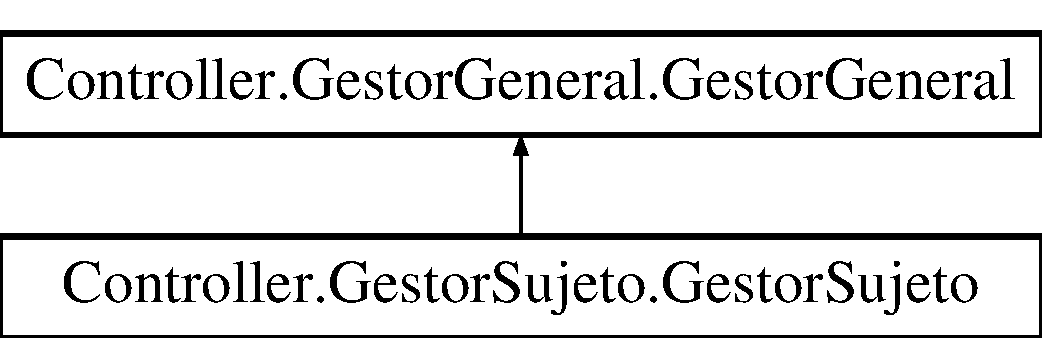
\includegraphics[height=2.000000cm]{class_controller_1_1_gestor_general_1_1_gestor_general}
\end{center}
\end{figure}


\subsection{Detailed Description}
\begin{DoxyVerb}classdocs
\end{DoxyVerb}
 

The documentation for this class was generated from the following file\+:\begin{DoxyCompactItemize}
\item 
Controller/Gestor\+General.\+py\end{DoxyCompactItemize}

\hypertarget{class_controller_1_1_gestor_sujeto_1_1_gestor_sujeto}{}\section{Controller.\+Gestor\+Sujeto.\+Gestor\+Sujeto Class Reference}
\label{class_controller_1_1_gestor_sujeto_1_1_gestor_sujeto}\index{Controller.\+Gestor\+Sujeto.\+Gestor\+Sujeto@{Controller.\+Gestor\+Sujeto.\+Gestor\+Sujeto}}
Inheritance diagram for Controller.\+Gestor\+Sujeto.\+Gestor\+Sujeto\+:\begin{figure}[H]
\begin{center}
\leavevmode
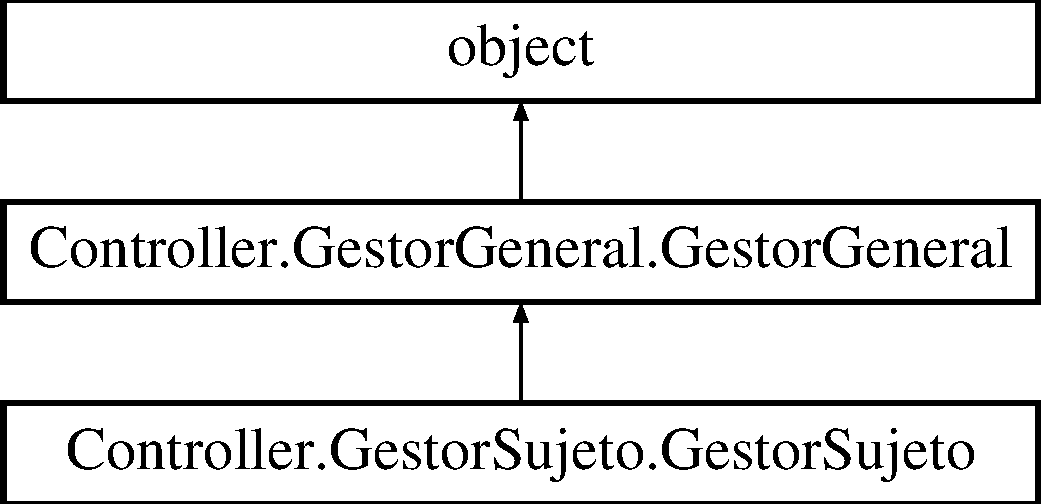
\includegraphics[height=3.000000cm]{class_controller_1_1_gestor_sujeto_1_1_gestor_sujeto}
\end{center}
\end{figure}
\subsection*{Public Member Functions}
\begin{DoxyCompactItemize}
\item 
def \hyperlink{class_controller_1_1_gestor_sujeto_1_1_gestor_sujeto_af03120d2a26ad27cf43979b059065818}{\+\_\+\+\_\+init\+\_\+\+\_\+} (self)
\end{DoxyCompactItemize}
\subsection*{Additional Inherited Members}


\subsection{Detailed Description}
\begin{DoxyVerb}classdocs
\end{DoxyVerb}
 

\subsection{Constructor \& Destructor Documentation}
\mbox{\Hypertarget{class_controller_1_1_gestor_sujeto_1_1_gestor_sujeto_af03120d2a26ad27cf43979b059065818}\label{class_controller_1_1_gestor_sujeto_1_1_gestor_sujeto_af03120d2a26ad27cf43979b059065818}} 
\index{Controller\+::\+Gestor\+Sujeto\+::\+Gestor\+Sujeto@{Controller\+::\+Gestor\+Sujeto\+::\+Gestor\+Sujeto}!\+\_\+\+\_\+init\+\_\+\+\_\+@{\+\_\+\+\_\+init\+\_\+\+\_\+}}
\index{\+\_\+\+\_\+init\+\_\+\+\_\+@{\+\_\+\+\_\+init\+\_\+\+\_\+}!Controller\+::\+Gestor\+Sujeto\+::\+Gestor\+Sujeto@{Controller\+::\+Gestor\+Sujeto\+::\+Gestor\+Sujeto}}
\subsubsection{\texorpdfstring{\+\_\+\+\_\+init\+\_\+\+\_\+()}{\_\_init\_\_()}}
{\footnotesize\ttfamily def Controller.\+Gestor\+Sujeto.\+Gestor\+Sujeto.\+\_\+\+\_\+init\+\_\+\+\_\+ (\begin{DoxyParamCaption}\item[{}]{self }\end{DoxyParamCaption})}



The documentation for this class was generated from the following file\+:\begin{DoxyCompactItemize}
\item 
Controller/\hyperlink{_gestor_sujeto_8py}{Gestor\+Sujeto.\+py}\end{DoxyCompactItemize}

%--- End generated contents ---

% Index
\backmatter
\newpage
\phantomsection
\clearemptydoublepage
\addcontentsline{toc}{chapter}{Index}
\printindex

\end{document}
